% Local numeric construction example, not source data. Replace every object.
% Compute derived coordinates first; preserve the actual original relations.
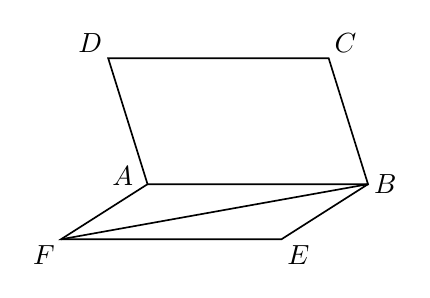
\begin{tikzpicture}[x=1cm,y=1cm,font=\normalsize,
 geometry edge/.style={solid,line width=.6pt},
 geometry mark/.style={solid,line width=.6pt},
 geometry label/.style={font=\normalsize,inner sep=2pt}]
\coordinate (A) at (1.2,1.0);
\coordinate (B) at (4.0,1.0);
\coordinate (C) at (3.5,2.6);
\coordinate (D) at (0.7,2.6);
\coordinate (E) at (2.9,0.3);
\coordinate (F) at (0.1,0.3);
\draw[geometry edge] (D)--(C)--(B)--(A)--cycle;
\draw[geometry edge] (A)--(F)--(E)--(B);
\draw[geometry edge] (F)--(B);
\node[geometry label,left,xshift=-3pt,yshift=3pt] at (A) {$A$};
\node[geometry label,right] at (B) {$B$};
\node[geometry label,above right] at (C) {$C$};
\node[geometry label,above left] at (D) {$D$};
\node[geometry label,below right] at (E) {$E$};
\node[geometry label,below left] at (F) {$F$};
\end{tikzpicture}
